\documentclass[../differential_methods.tex]{subfiles}
\begin{document}
\section{Aula 18 - 10 de Junho, 2026}
\subsection{Motivações}
\begin{itemize}
	\item Equação de Advecção
\end{itemize}
\subsection{Equações Hiperbólicas}
Começamos o tópico das equações para sistemas hiperbólicos, que apesar de ser simples no caso unidimensional e com problema de Cauchy, passa a ter complexidade considerável com mudanças nessas condições, vide Navier-Stokes
\[
	\underbrace{\frac{\partial^{}u}{\partial t^{}} + \underline{u}\cdot \nabla \nabla \underline{u}}_{\text{Parte hiperbólica}}= -\nabla p + \mu \nabla \cdot (\nabla \underline{u} + \nabla \underline{u}^{T})
\]
A parte hiperbólica, correspondente ao transporte, é o termo mais complicador de Navier-Stokes.

Começamos com um problema simples, chamado \textbf{equação de advecção}, por enquanto como problema de Cauchy:
\[
	u_t + au_x = 0, \quad -\infty<x<\infty, \quad t>0,\quad u(x, 0) = \eta (x),
\]
onde a seria um termo que representa a ``velocidade de transporte''; para uma breve revisão do aspecto analítico dela, vamos considerar \(x = x(s), \; t = t(s)\) tal que \(u(x, t) = u(x(s), t(s))\). Pela regra da cadeia,
\[
	\frac{\partial^{}u}{\partial s^{}} = \frac{\partial^{}u}{\partial x^{}}\frac{\partial^{}x}{\partial s^{}} + \frac{\partial^{}u}{\partial t^{}}\frac{\partial^{}t}{\partial s^{}}=0,
\]
que é essencialmente a equação de transporte se \(\partial_{s}x = a\) e \(\partial_s t = 1\). Logo,
\[
	x(s) = x_{0} + as \quad\&\quad t(s) = t_{0} + s,
\]
que são as \textit{curvas características} da equação transporte -- com estas identificações, a equação representa o transporte de algum perfil inicial ao longo do tempo e do espaço.
\begin{figure}[H]
	\begin{center}
		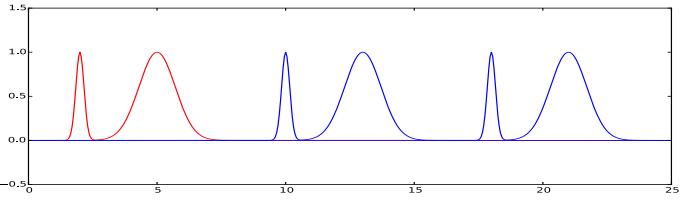
\includegraphics[height=\textheight, width=\textwidth, keepaspectratio]{./Images/transport_equation_18.png}
	\end{center}
	\caption{a linha vermelha foi transportada ao longo do espaço a cada tempo.}
\end{figure}

Agora, como \(\partial_s u = 0\), sabemos que \(u(x, t)\) deve ser constante para qualquer s! Por isso, para \(s=0\), deve acontecer
\begin{align*}
	\mathrm{cte} = u(x(s), t(s)) & = u(x_{0}+as, s)                          \\
	                             & = u(x_{0}, 0)     \text{   (usando s=0)}  \\
	                             & = \eta (x_{0})                            \\
	                             & = \eta (x_{0}-as)                         \\
	                             & = \eta (x_{0}-at) \text{   (usando t=s)},
\end{align*}
que é a condição inicial transladada \(at\) unidades para a direita. As curvas características são, então, as direções de propagação de informações das equações hiperbólicas!

Se tivermos uma equação da forma
\[
	u_t + au_x + bu = d,
\]
podemos obter
\[
	\frac{\mathrm{d}x}{\mathrm{d}t} = a \Rightarrow \frac{\mathrm{d}u}{\mathrm{d}t} = d - b_u,
\]
ou então, por exemplo,
\[
	u_t + tu_x = 3 \Rightarrow \frac{\mathrm{d}x}{\mathrm{d}t} = t \Rightarrow  x(t)=\frac{t^{2}}{2}+x_{0}.
\]

Com nosso conhecimento de discretização, iremos discretizar a equação hiperbólica e ver o que podemos obter! Partindo de
\[
	u_t + au_x = 0,
\]
o primeiro passo é discretizar no tempo por \(\Delta t\) (ou k) e no espaço por \(\Delta x\) (ou h), obtendo pares \((x_{j}, t_{n}) = (jh, nk)\). Usando uma aproximação de diferenças finitas e diferenças centrais para
\[
	u_t(x_{j}, t_{n}) + a u_x(x_{j}, t_{n}) = 0,
\]
segue que
\[
	u_t(x_{j}, t_{n}) \approx \frac{u(x_{j}, t_{n}+\Delta t) - u(x_{j}, t_{n})}{\Delta t} + \mathcal{O}(\Delta t)
\]
e
\[
	u_x(x_{j}, t_{n})\approx \frac{u(x_{j}+\Delta x, t_{n}) - u(x_{j}-\Delta x, t_{n})}{2\Delta x} + \mathcal{O}(\Delta x^{2}),
\]
tal que, denotando por \(U_{j}^{n}\approx u(x_{j}, t_{n})\), obtemos o método
\[
	\frac{U_{j}^{n+1} - U_{j}^{n}}{\Delta t} + a \frac{U_{j+1}^{n} - U_{j-1}^{n}}{2\Delta x} = 0,
\]
que é de consistência à ordem \(\mathcal{O}(\Delta t + \Delta x^{2})\). Resta analisarmos a convergência dele, que vai ser a estabilidade (já temos a consistência), podendo ser feito por Von-Neumann isolando o termo do passo temporal n+1:
\[
	U_{j}^{n+1} = U_{j}^{n} - a \frac{\Delta t}{2\Delta x}(U_{j+1}^{n} - U_{j-1}^{n}).
\]
Denotando \(\xi h \eqqcolon \beta \) e usando \(U_{j}^{n} = e^{ijh\xi } =e^{i\beta j}\), comparamos a expressão acima com
\[
	U_{j}^{n+1} = g(\xi ) U_{j}^{n},
\]
tal que
\[
	g e^{i\beta j} = e^{i\beta j} - \frac{a\Delta t}{2\Delta x}\biggl(e^{i\beta (j+1)} - e^{i\beta (j-1)}\biggr) = e^{i\beta j}\biggl(1 - \frac{a\Delta t}{2\Delta x}(e^{i\beta }- e^{-i\beta })\biggr),
\]
e obtemos
\[
	g = 1 - \frac{a\Delta t}{2\Delta x}(e^{i\beta } - e^{-i\beta }) = 1- \frac{a\Delta t}{2\Delta x}2i \sin^{}{\beta }=1-\frac{a\Delta t}{\Delta x}i\sin^{}{\beta }.
\]
Agora, analisamos o módulo de g, de modo que
\[
	| g |^{2} = 1 + \biggl(\frac{a\Delta t}{\Delta x}\biggr)^{2} \sin^{2}{\beta },
\]
mas como a norma é sempre maior que 1, \textbf{o método é incondicionalmente instável}! Não adianta usar o método mais simples, porque ele não vai convergir. E agora?

O próximo passo natural é partir para um método diferente, especificamente o \hypertarget{lax_friedrichs}{\textbf{método Lax-Friedrichs}}, que consiste em trocar o termo \(U_{j}^{n}\) da discretização por uma média entre dois espaços:
\[
	\boxed{U_{j}^{n+1} = \frac{1}{2}(U_{j-1}^{n} + U_{j+1}^{n}) - \frac{a\Delta t}{2\Delta x}(U_{j+1}^{n} + U_{j-1}^{n})}
\]
Repetindo a análise de Von-Neumann para este caso, observar-se-á que
\[
	g = \frac{1}{2}(e^{i\beta } + e^{-i\beta }) - \frac{a\Delta t}{2\Delta x}(e^{i\beta } - e^{-i\beta }) = \cos^{}{\beta } - \frac{a\Delta t}{\Delta x}i\sin^{}{\beta },
\]
o qual é um número complexo dentro de um círculo, cujo raio será menor que 1 se, e somente se, o termo \((a\Delta t)/\Delta x\) tiver módulo menor ou igual a 1! Agora sim, temos um método condicionalmente estável e com condição de estabilidade dada por
\[
	\frac{| a |\Delta t}{\Delta x} \leq 1;
\]
o termo à esquerda é chamado \textbf{número de Courant}.

Com essa pequena modificação, conseguimos um método com custo computacional de um método explícito, convergente desde que \(\Delta t\) e \(\Delta x\) tenham a mesma ordem de convergência, que não é uma restrição severa!
\begin{exr}
	Calcule o erro de truncamento do \hyperlink{lax_friedrichs}{\textit{método Lax-Friedrichs}}.
\end{exr}

Em suma, o que fizemos até agora foi testar uma discretização central, que foi instável, e uma pequena modificação nele garantiu uma estabilidade condicional. Em seguida, vamos convencionar \(a > 0\), tornando as características em retas que levam a informação da esquerda à direita; o método que fizemos, essencialmente, pega informação em formato de T invertido -- o (n+1)-ésimo passo temporal usa o (j-1), o (j+1) e o j-ésimo passos temporais no tempo n. Compor a solução acima consiste em pegar informação à esquerda e à direita! O primeiro faz sentido pela forma que a informação se propaga, mas o segundo não! Então, fazer um estêncil simétrico talvez não seja a melhor coisa aqui, pois a informação à direita ainda nem existe às vezes.
Logo, usaremos uma discretização regressiva para o termo derivado em x:
\[
	u_x \approx a \frac{u(x_{j}, t_{n}) - u(x_{j}-\Delta x, t_{n})}{\Delta x} + \mathcal{O}(\Delta x),
\]
dando o \textbf{método \textit{upwind}} para propagações da esquerda à direita da forma
\[
	\frac{U_{j}^{n+1}-U_{j}^{n}}{\Delta t} + a \frac{U_{j}^{n} - U_{j-1}^{n}}{\Delta x} = 0;
\]
por outro lado, se \(a < 0\), o sentido de propagação passa a ser da direita para a esquerda, sendo então preciso um método progressivo em x:
\[
	u_{x} \approx a \frac{u(x_{j}+\Delta x, t_{n}) - u(x_{j}, t_{n})}{\Delta x}+\mathcal{O}(\Delta x),
\]
do qual obtemos o \textbf{método \textit{downwind}} para o transporte
\[
	\frac{U_{j}^{n+1} - U_{j}^{n}}{\Delta t} + a \frac{U_{j+1}^{n} - U_{j}^{n}}{\Delta x} = 0.
\]
\begin{exr}
	Determine se os métodos acima convergem ou não. \textbf{Dica:} a consistência é da ordem \(\mathcal{O}(\Delta t+ h)\), e a análise de Von-Neumann tem que dar a mesma condição de antes no número de Courant.
\end{exr}
De forma compacta,
\[
	U_{j}^{n+1} = \left\{\begin{array}{ll}
		U_{j}^{n} - \frac{a \Delta t}{\Delta x}(U_{j}^{n} - U_{j-1}^{n}), & \quad a \geq 0 \\
		U_{j}^{n} - \frac{a\Delta t}{\Delta x}(U_{j+1}^{n} - U_{j}^{n}),  & \quad a < 0
	\end{array}\right..
\]

Normalmente, não queremos resolver o método em um espaço infinito, então costuma ser bom limitar o intervalo, por exemplo, a um espaço \([0, 1]\), resolvendo até certo tempo T, sendo necessário impôr apenas uma condição de contorno pela unidimensionalidade; onde ela deve ser posta? Depende de cada problema; se o transporte é da esquerda pra direita, coloca à esquerda, no 0, mas se ela for da direita pra esquerda, então tem que pôr a condição à direita, no 1.
Porém, considerando o primeiro caso, surge um problema: ao chegar no limite à direita, fica faltando um ponto para descrever o problema! Por isso acaba sendo vantajoso usar métodos unilaterais ao invés dos simétricos, mesmo sendo possível ajustar a condição de contorno no limite, afinal isso acaba adicionando erros ao método. Uma solução mais ingênua que aparece às vezes é considerar uma condição de contorno fictícia, por exemplo que o que está saindo não é pra ser mexido, impondo a condição 0.
\begin{def*}
	O lado por onde o escoamento entra é chamado \textbf{inflow}, e o lado por onde sai é chamado \textbf{outflow} (se vai estar à esquerda ou à direita depende do sinal do a). \(\square\)
\end{def*}
O caso de \(a < 0\) é análogo.

\end{document}
